\documentclass{beamer}
\usetheme{Berkeley}

\title{Introduction to NoSQL Databases}
\author{Skill Networks and Coursera}
\date{\today}

\begin{document}

\frame{\titlepage}

\section{Overview of NoSQL}

\begin{frame}{\centering Overview of NoSQL}
\centering
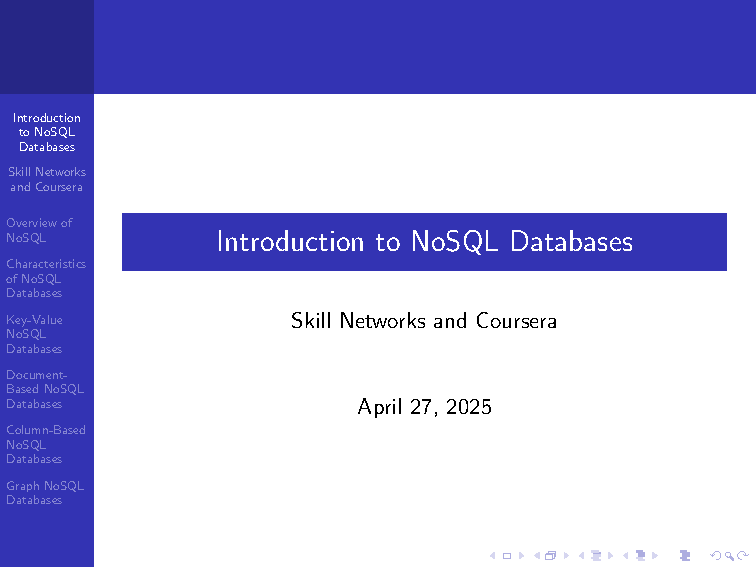
\includegraphics[width=0.7\linewidth]{figures/nosql}
\end{frame}

\begin{frame}{What is NoSQL?}
\begin{itemize}
    \item NoSQL = Not Only SQL
    \item Family of non-relational databases
    \item Flexible schemas, designed for modern applications
    \item Provide horizontal scalability, fault tolerance, and availability
\end{itemize}
\end{frame}

\begin{frame}{History of NoSQL}
\begin{itemize}
    \item 1970-2000: Dominated by relational databases
    \item 2000s: Internet boom -> need for high scalability and availability
    \item Innovations: Google's MapReduce, Amazon's Dynamo
    \item Emergence of open-source NoSQL databases: Cassandra, MongoDB, CouchDB, HBase
\end{itemize}
\end{frame}

\begin{frame}{Why NoSQL?}
\begin{itemize}
    \item Flexible data models (unstructured, semi-structured data)
    \item Horizontal and vertical scalability
    \item High availability and fault tolerance
    \item Designed for distributed environments
\end{itemize}
\end{frame}

\section{Characteristics of NoSQL Databases}

\begin{frame}{\centering Characteristics of NoSQL Databases}
\centering
\includegraphics[width=0.7\linewidth]{figures/nosql_benefits_diagram}
\end{frame}

\begin{frame}{Characteristics of NoSQL}
\begin{itemize}
    \item Non-relational architecture
    \item Open-source origins
    \item Specialized for specific use cases
    \item Flexible schemas for agile development
\end{itemize}
\end{frame}

\begin{frame}{Benefits of NoSQL}
\begin{itemize}
    \item Scalability (elastic horizontal scaling)
    \item Performance (low latency with high concurrency)
    \item High availability (distributed replication)
    \item Cost-efficient (cloud and commodity hardware)
    \item Flexible schemas and intuitive data models
\end{itemize}
\end{frame}

\section{Key-Value NoSQL Databases}

\begin{frame}{\centering Key-Value NoSQL Databases}
\centering
\includegraphics[width=0.6\linewidth]{figures/key_value_diagram}
\end{frame}

\begin{frame}{Key-Value Databases}
\begin{itemize}
    \item Data stored as key and opaque value blob
    \item Simple CRUD operations
    \item Highly scalable and easily sharded
    \item Examples: Amazon DynamoDB, Redis, Oracle NoSQL
\end{itemize}
\end{frame}

\begin{frame}{Key-Value Use Cases}
\begin{itemize}
    \item Session management
    \item User profile storage
    \item Shopping cart data
\end{itemize}
\end{frame}

\section{Document-Based NoSQL Databases}

\begin{frame}{\centering Document-Based NoSQL Databases}
\centering
\includegraphics[width=0.6\linewidth]{figures/document_db_diagram}
\end{frame}

\begin{frame}{Document Databases}
\begin{itemize}
    \item Extends key-value model with visible, queryable documents
    \item Flexible schema (JSON, XML)
    \item Horizontal scalability and indexing support
    \item Examples: MongoDB, CouchDB, IBM Cloudant
\end{itemize}
\end{frame}

\begin{frame}{Document Use Cases}
\begin{itemize}
    \item Event logging
    \item Blogging platforms
    \item Operational datasets for web/mobile apps
\end{itemize}
\end{frame}

\section{Column-Based NoSQL Databases}

\begin{frame}{\centering Column-Based NoSQL Databases}
\centering
\includegraphics[width=0.6\linewidth]{figures/column_family_diagram}
\end{frame}

\begin{frame}{Column-Based Databases}
\begin{itemize}
    \item Inspired by Google's Bigtable
    \item Store data in columns grouped into families
    \item Ideal for large, sparse datasets
    \item Examples: Cassandra, HBase, Accumulo
\end{itemize}
\end{frame}

\begin{frame}{Column Use Cases}
\begin{itemize}
    \item Data warehousing and business intelligence
    \item IoT data management
    \item Financial and scientific analysis
\end{itemize}
\end{frame}

\section{Graph NoSQL Databases}

\begin{frame}{\centering Graph NoSQL Databases}
\centering
\includegraphics[width=0.6\linewidth]{figures/graph_db_diagram}
\end{frame}

\begin{frame}{Graph Databases}
\begin{itemize}
    \item Store entities (nodes) and relationships (edges)
    \item Efficient for traversing highly connected data
    \item ACID-compliant
    \item Examples: Neo4j, ArangoDB, Amazon Neptune
\end{itemize}
\end{frame}

\begin{frame}{Graph Use Cases}
\begin{itemize}
    \item Social networking
    \item Routing and spatial applications
    \item Recommendation engines
\end{itemize}
\end{frame}

\end{document}
